\documentclass{ctexart}
\usepackage[left=2cm,right=2cm,top=2cm,bottom=1.5cm]{geometry}
\usepackage{xeCJK}
\usepackage{hyperref}
\usepackage{xcolor}
\usepackage{minted}
\usepackage{graphicx}
\usepackage{amsmath}
\usepackage{fancyhdr}
\usepackage{blindtext}
 
\xeCJKsetup{CJKmath=true}   % 开启公式中的中文显示
% \setCJKmainfont{KaiTi}
\hypersetup{colorlinks=true,linkcolor=blue,filecolor=magenta,urlcolor=cyan} % set the hyperref's link color
% \ctexset{section/number = \Chinese{section}} % 设置中文标题

% define some custom colors
\definecolor{grey100}{HTML}{F5F5F5}

\newcommand{\monospace}[2][grey100]{\colorbox{#1}{\texttt{#2}}} % define new command monospace

\begin{document}
\begin{titlepage}
    \begin{center}

        \vspace*{4cm}

        \Huge
        \textbf{“银行业务管理系统”}


        \vspace{4cm}

        \LARGE
        \textbf{系统设计与实现报告}

        \vspace{3cm}

        \Large
        \textbf{姓名:Ezekiel B. Ouedraogo}

        \textbf{学号:PL19215001}

        \vspace{4cm}

        \textbf{计算机科学与技术学院}

        \textbf{中国科学技术大学}

        \textbf{2022年4月}
    \end{center}
\end{titlepage}


\tableofcontents
\section{概述}

\subsection{系统目标}

本系统旨在为某银行开发一个银行业务管理系统。
系统要求使用 MySQL 作为后端的 DBMS, 前端开发发工具不限。
于是我们使用了 B/S 架构,前端使用 React 开发并以 Flask 完成前后端通信。
该系统要求实现客户管理、账户管理、贷款管理和业务统计等功能。 

\subsection{需求说明}

银行有多个支行。各个支行位于某个城市,每个支行有唯一的名字。银行要监控每个支
行的资产。 银行的客户通过其身份证号来标识。银行存储每个客户的姓名、联系电话以及
家庭住址。为了安全起见,银行还要求客户提供一位联系人的信息,包括联系人姓名、手机
号、Email 以及与客户的关系。客户可以有帐户,并且可以贷款。客户可能和某个银行员工
发生联系,该员工是此客户的贷款负责人或银行帐户负责人。 银行员工也通过身份证号来
标识。员工分为部门经理和普通员工,每个部门经理都负责领导其所在部门的员工,并且每
个员工只允许在一个部门内工作。每个支行的管理机构存储每个员工的姓名、电话号码、家
庭地址、所在的部门号、部门名称、部门类型及部门经理的身份证号。银行还需知道每个员
工开始工作的日期,由此日期可以推知员工的雇佣期。银行提供两类帐户一储蓄帐户和支
票帐户。帐户可以由多个客户所共有,一个客户也可开设多个账户,但在一个支行内最多只
能开设一个储蓄账户和一个支票账户。每个帐户被赋以唯一的帐户号。银行记录每个帐户的
余额、开户日期、开户的支行名以及每个帐户所有者访问该帐户的最近日期。另外,每个储
蓄帐户有利率和货币类型,且每个支票帐户有透支额。 每笔贷款由某个分支机构发放,能
被一个或多个客户所共有。每笔贷款用唯一的贷款号标识。银行需要知道每笔贷款所贷金额
以及逐次支付的情况(银行将贷款分几次付给客户)。虽然贷款号不能唯一标识银行所有为
贷款所付的款项,但可以唯一标识为某贷款所付的款项。对每次的付款需要记录日期和金
额。

\subsection{本报告的主要贡献}

本报告详述了本银行管理系统的总体设计、 数据库设计、 前端设计、 后端适配设计、 前后端连接方式等、 内容详尽、 应有尽有。

\section{总体设计}

\subsection{系统模块结构}

\begin{figure}[H]
    \centering
    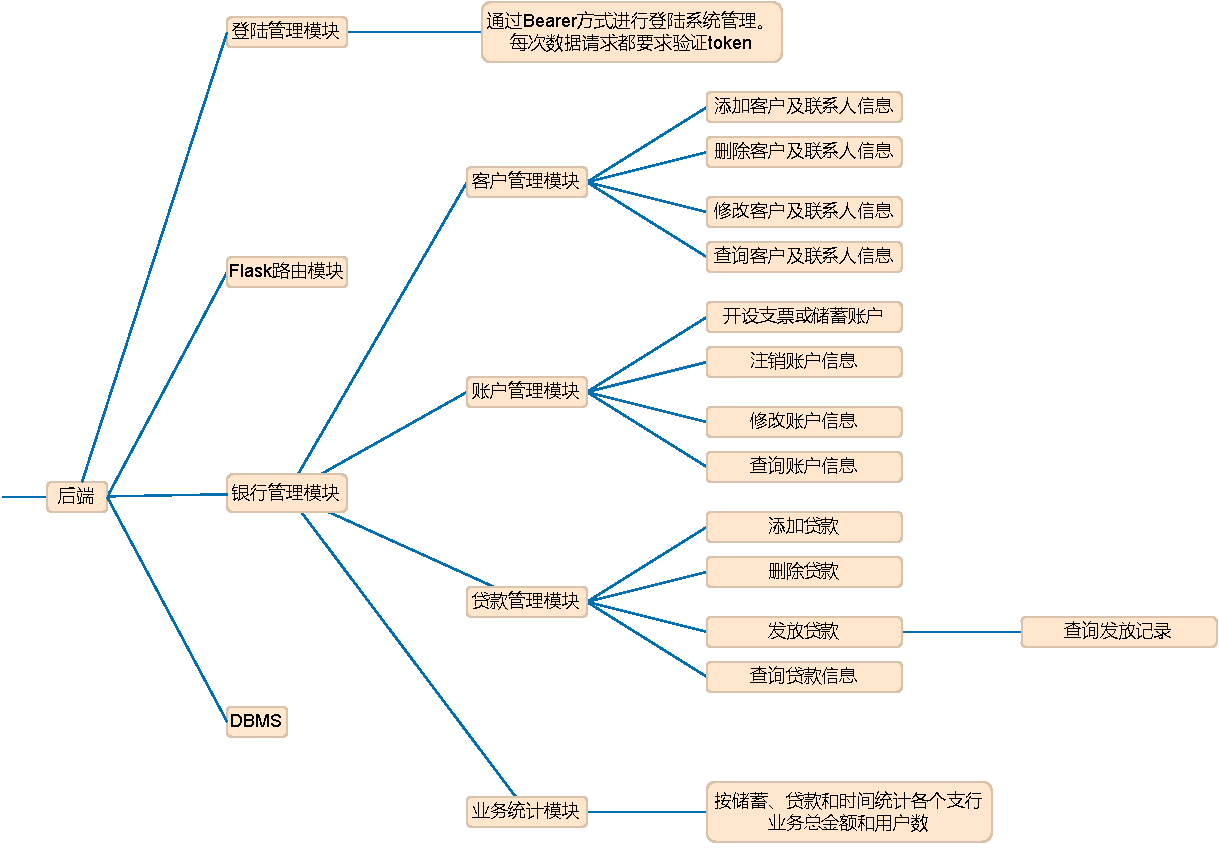
\includegraphics[width=\textwidth]{assets/diagram.drawio.pdf}
    \caption{后端设计}
\end{figure}

前端设计类似。

\subsection{系统工作流程}

\subsection{数据库设计}

ER图见\ref{fig:er-diagram}、物理数据库模型见\ref{fig:er-phys-diagram}。

\begin{figure}[H]
    \centering
    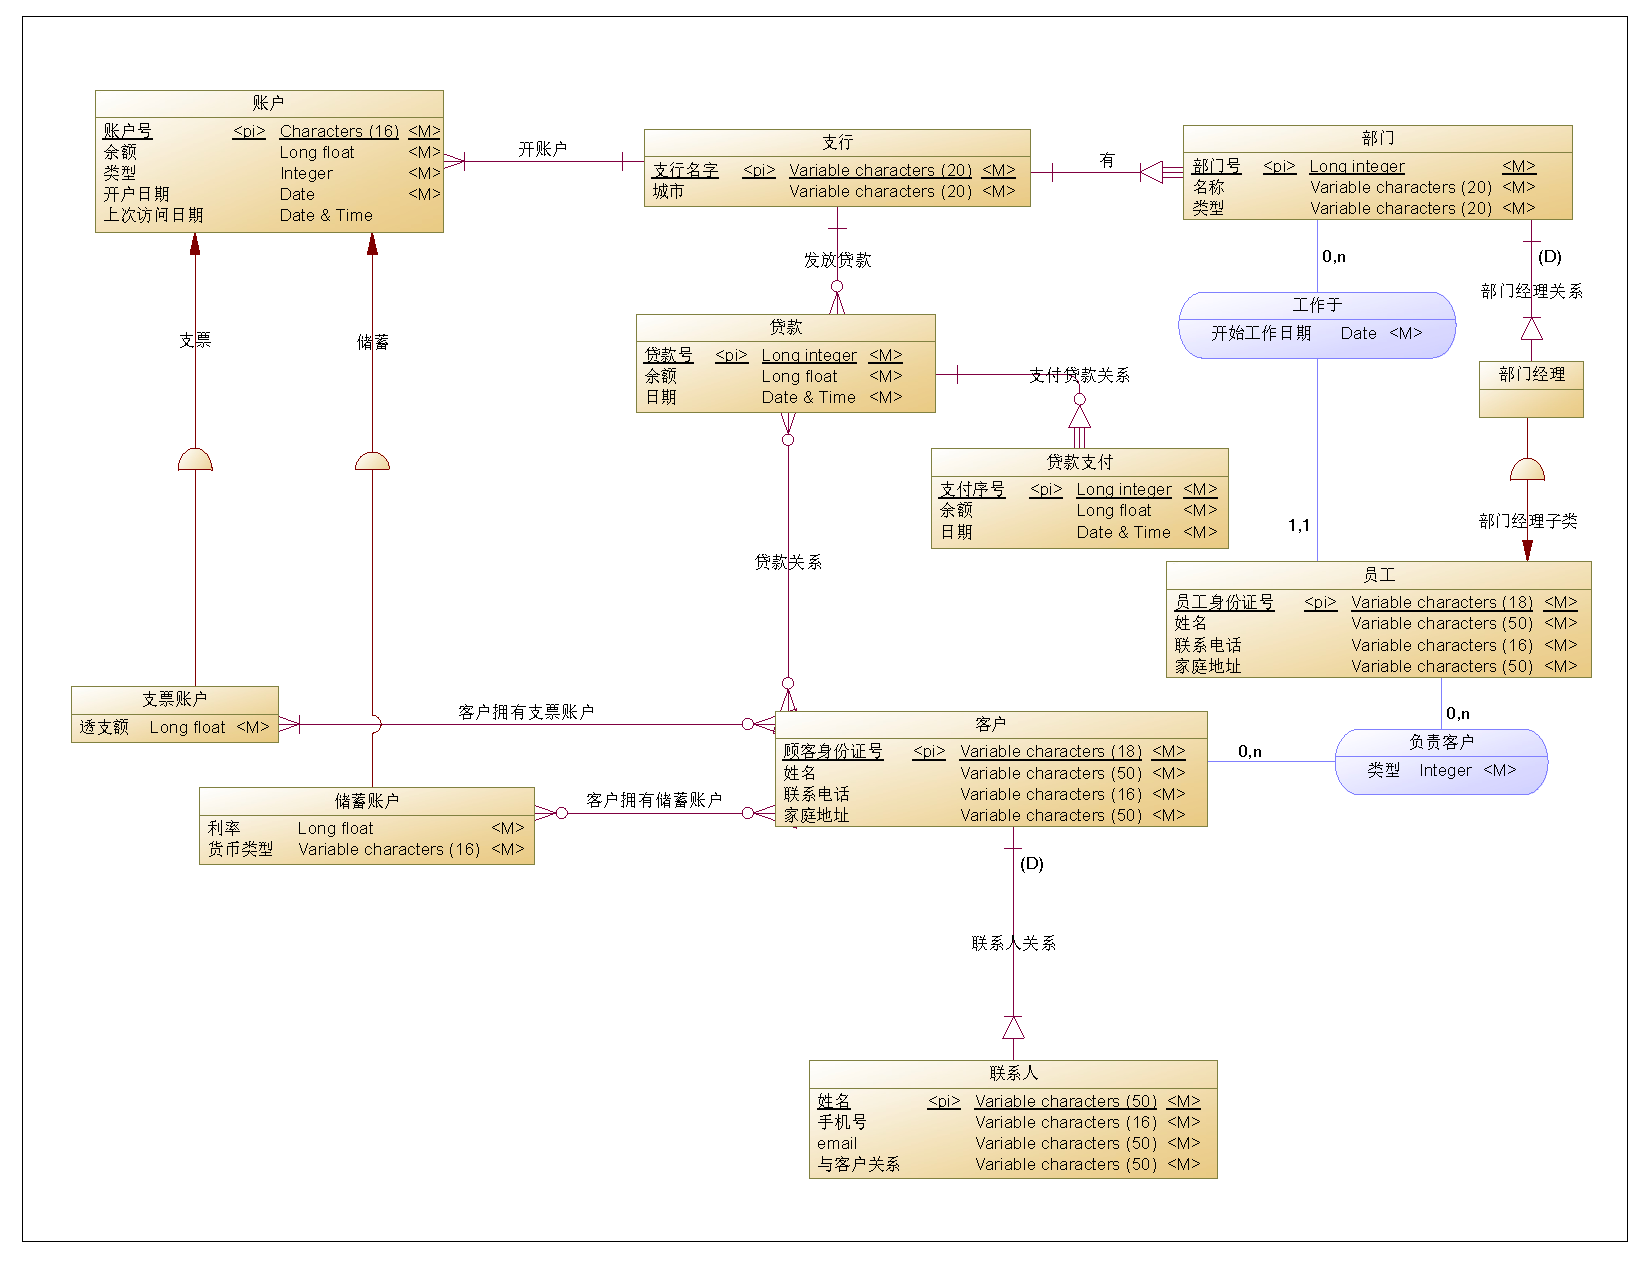
\includegraphics[width=0.8\textwidth]{assets/er-diagram.pdf}
    \caption{ER图}
    \label{fig:er-diagram}
\end{figure}

\begin{figure}[H]
    \centering
    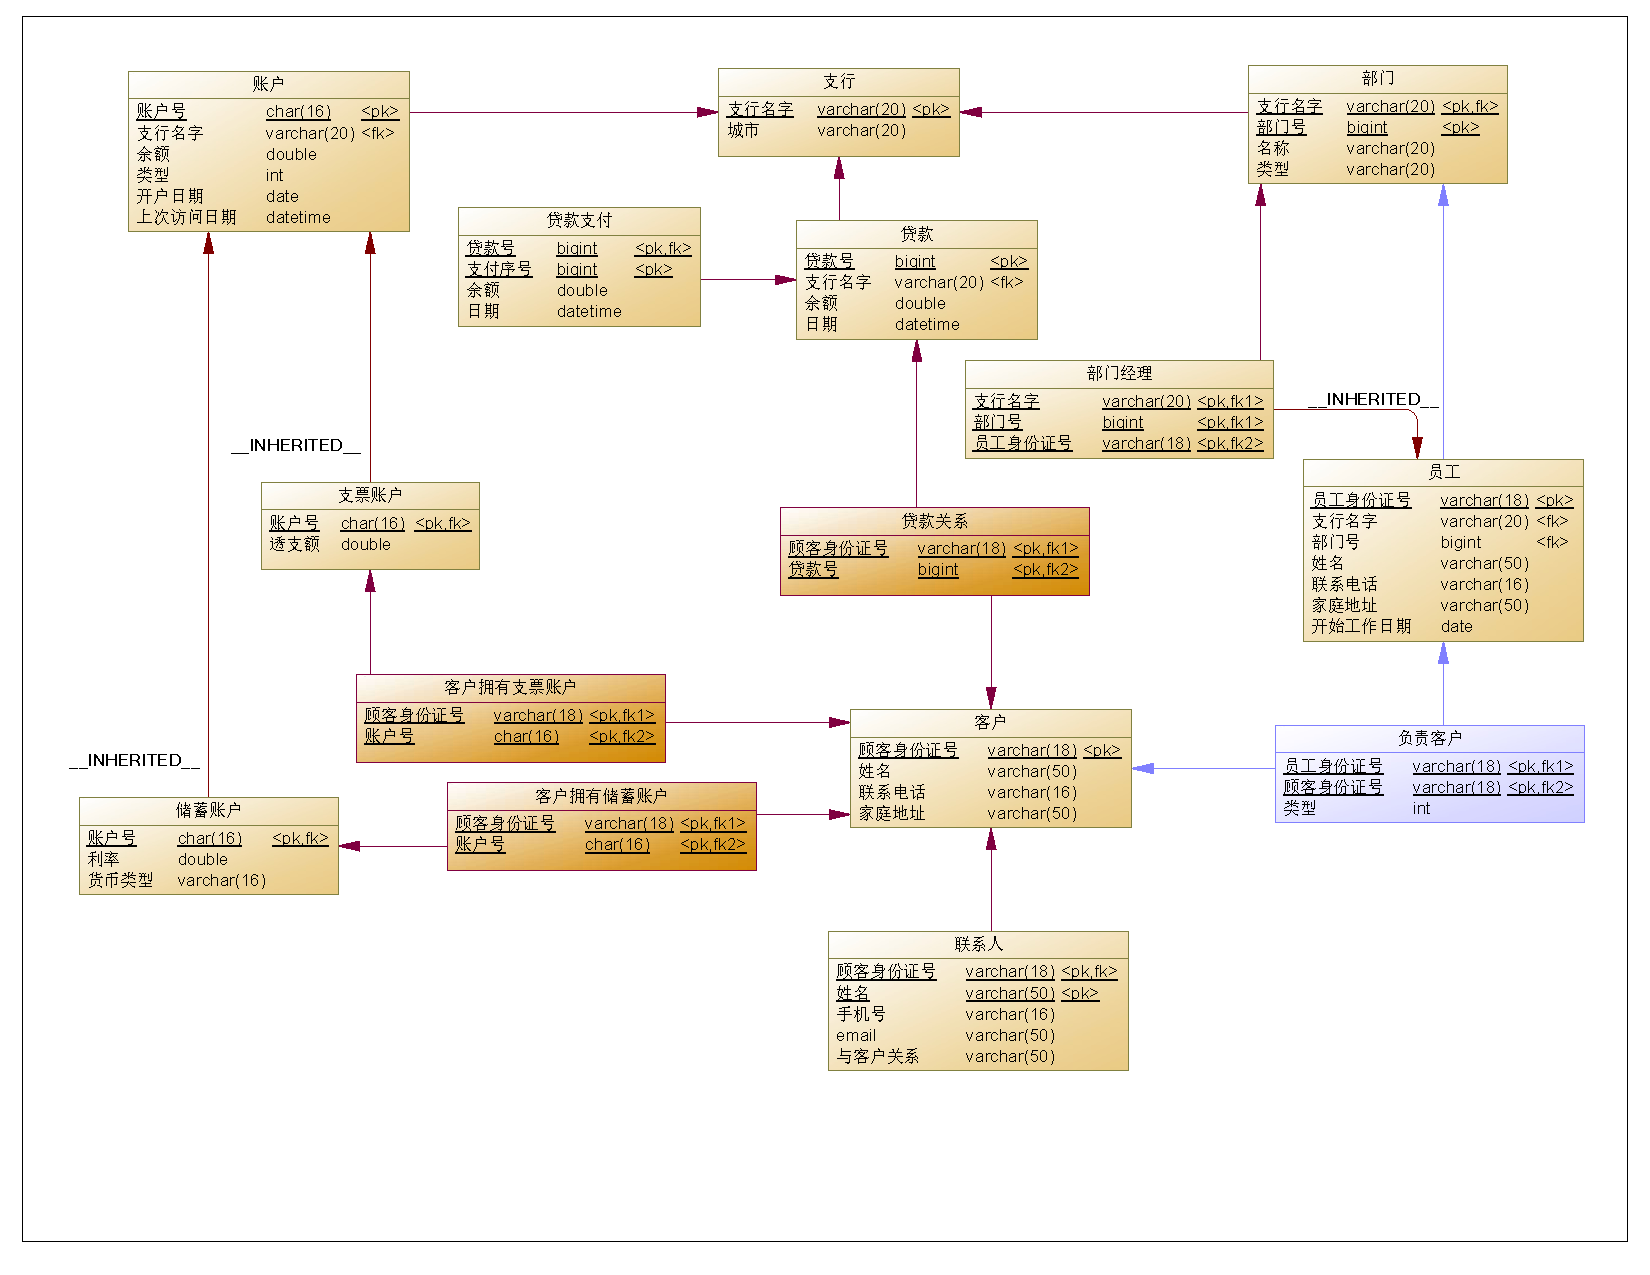
\includegraphics[width=0.8\textwidth]{assets/er-phys-diagram.pdf}
    \caption{物理数据库模型}
    \label{fig:er-phys-diagram}
\end{figure}

\section{实现与测试}

\begin{enumerate}
    \item 登录模块 ("/login")
    
    登陆后将从后端收到的token保存在本地。 后续向服务器发送请求时,将token放在请求头中。

    \begin{figure}[H]
        \centering
        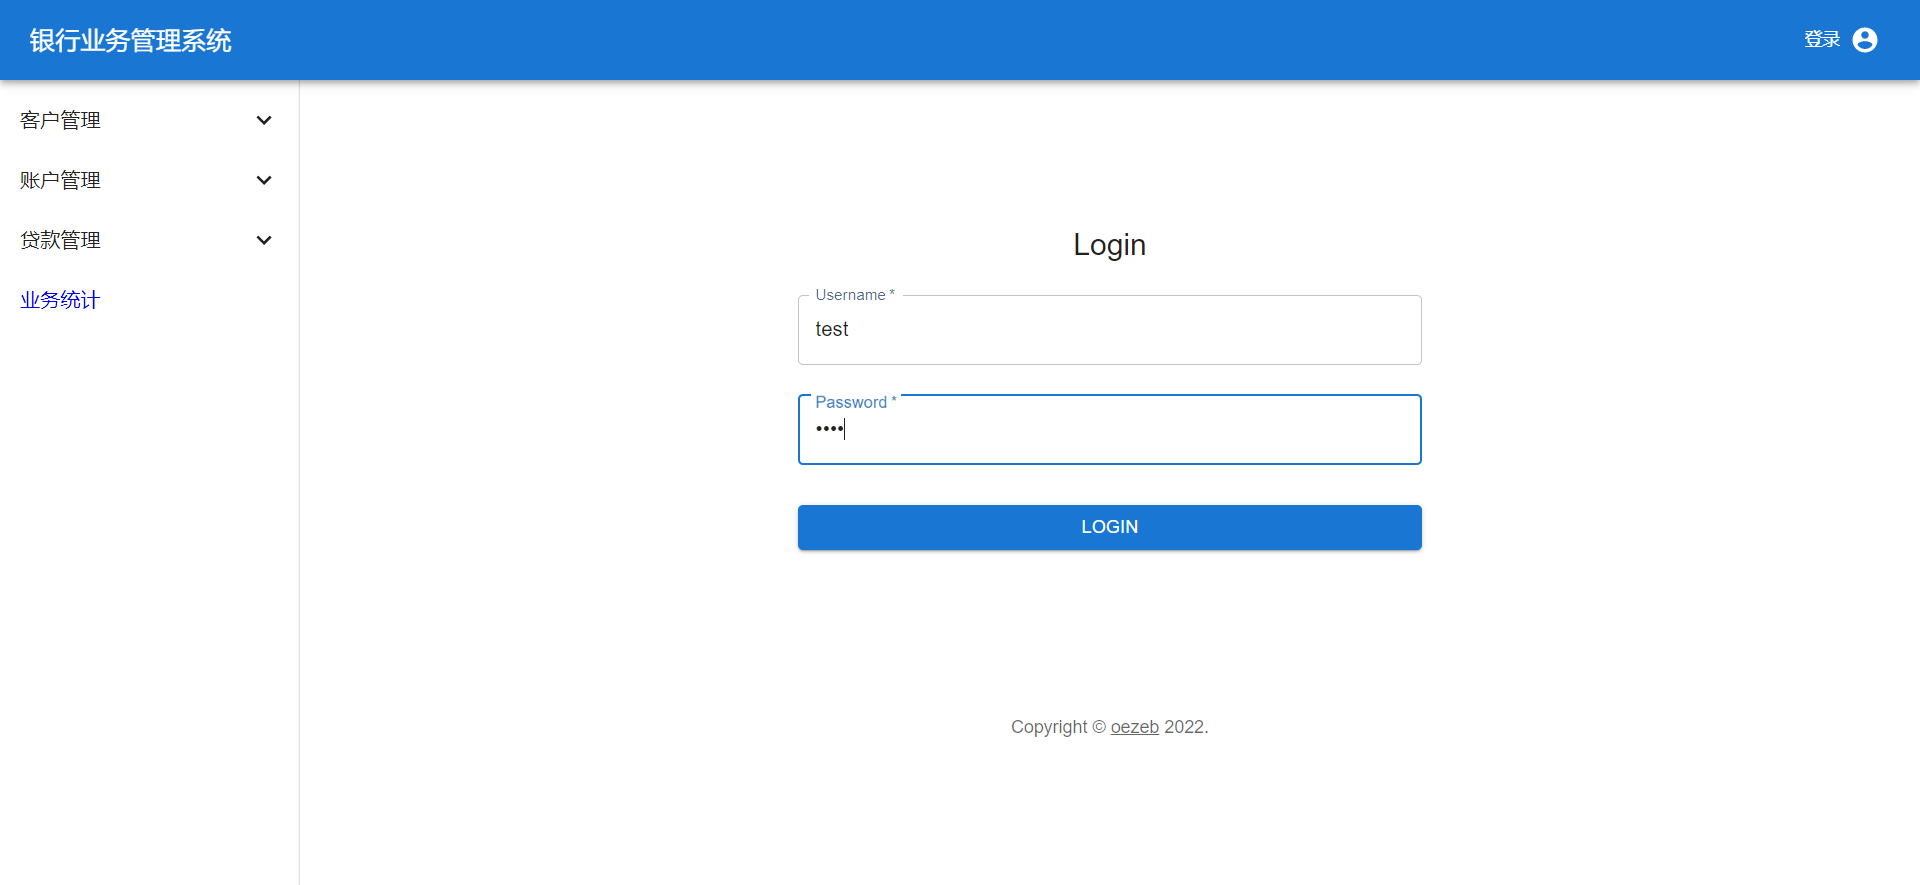
\includegraphics[width=\textwidth]{assets/images/login.png}
    \end{figure}

    \item 业务统计模块 ("/)
    
    根据选的支行,显示按业务分类(储蓄、贷款)和时间(月、季、年)统计业务总金额和用户数表格。

    \begin{figure}[H]
        \centering
        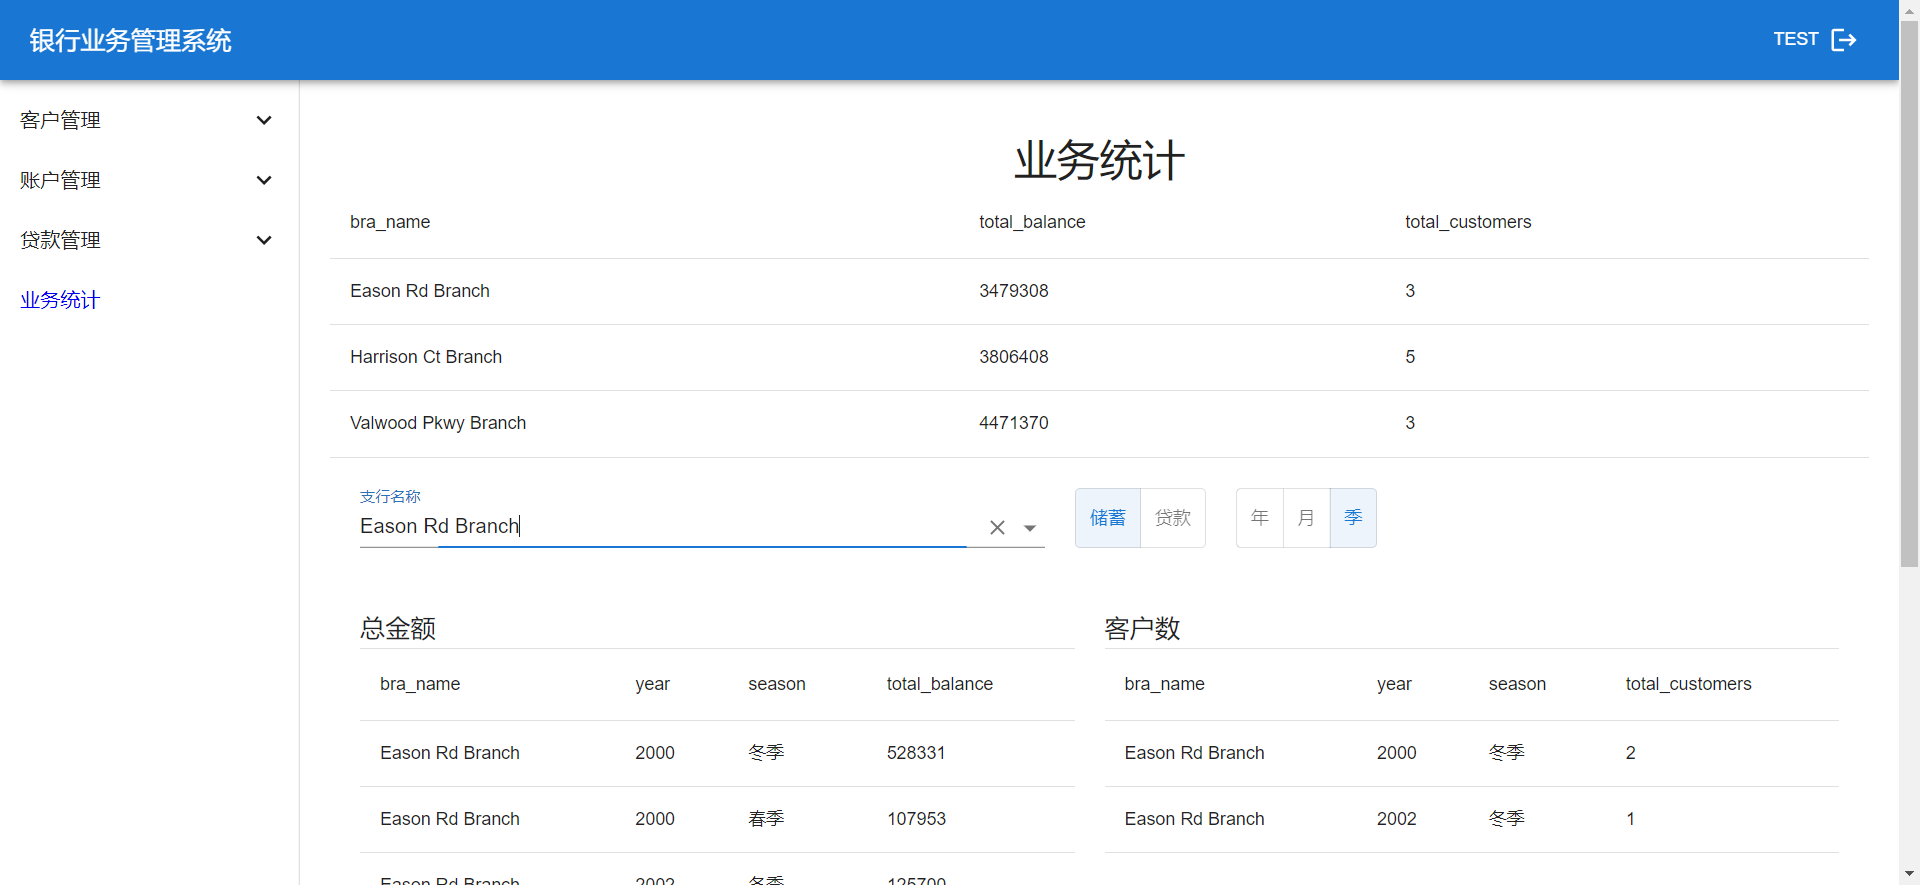
\includegraphics[width=\textwidth]{assets/images/dashboard.png}
    \end{figure}

    
    \item 客户管理模块
    
    \begin{enumerate}
        \item 增加客户模块 ("/add-customer")
        
        填客户及其联系人信息,并提交。

        \begin{figure}[H]
            \centering
            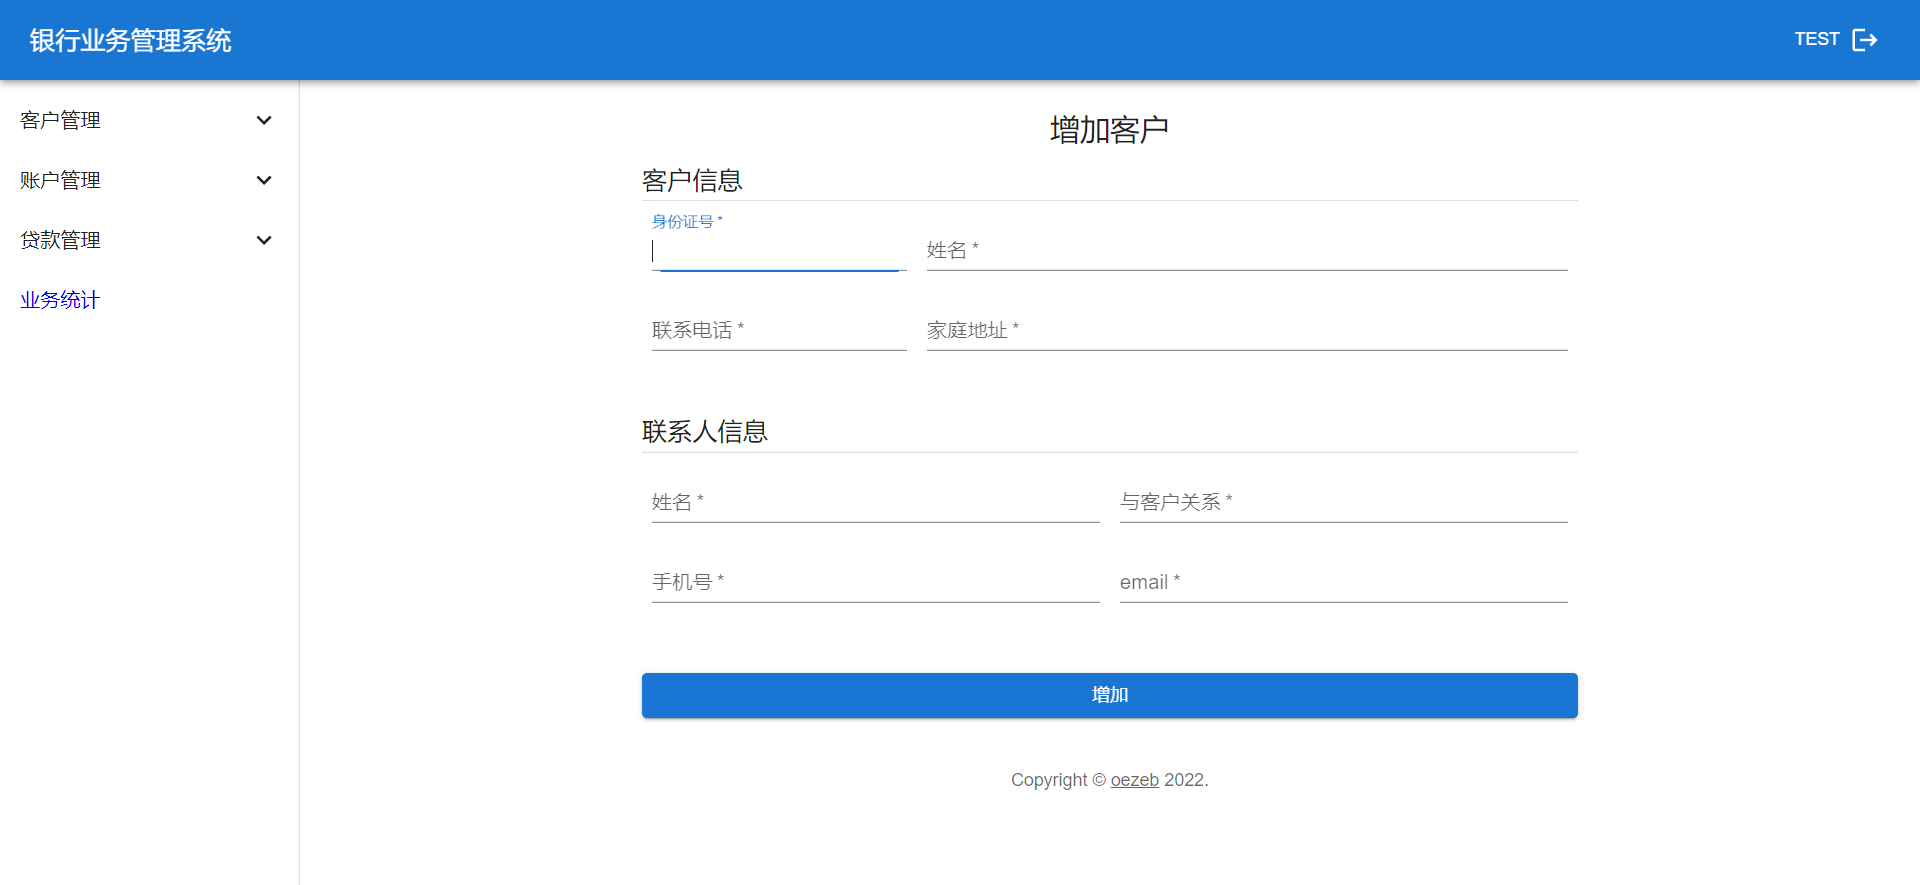
\includegraphics[width=\textwidth]{assets/images/add-customer.png}
        \end{figure}

        \item 修改客户信息模块 ("/edit-customer")
        
        选择客户后,其信息自动填充到表单中。修改客户信息,并提交。

        \begin{figure}[H]
            \centering
            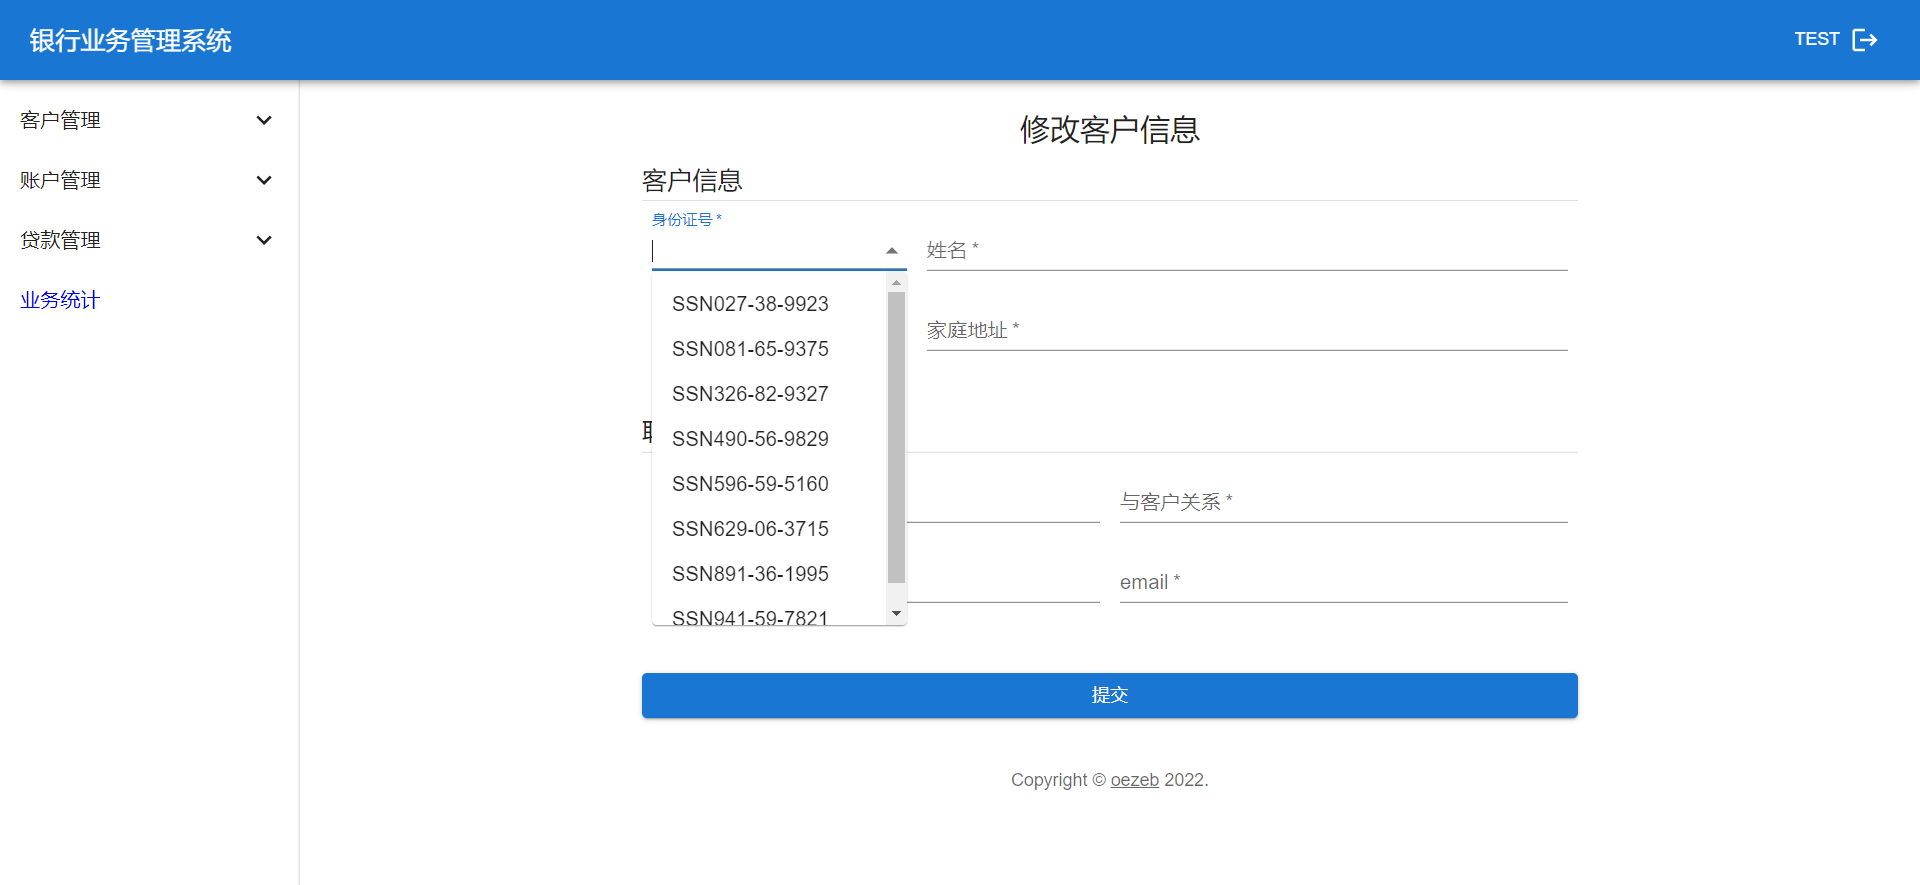
\includegraphics[width=\textwidth]{assets/images/edit-customer.png}
        \end{figure}

        \item 查询客户信息模块 ("/customer-info")
        
        根据客户身份证号或客户名称查询客户信息。结果列表中可以通过“actions”列的按钮删除客户。

        \begin{figure}[H]
            \centering
            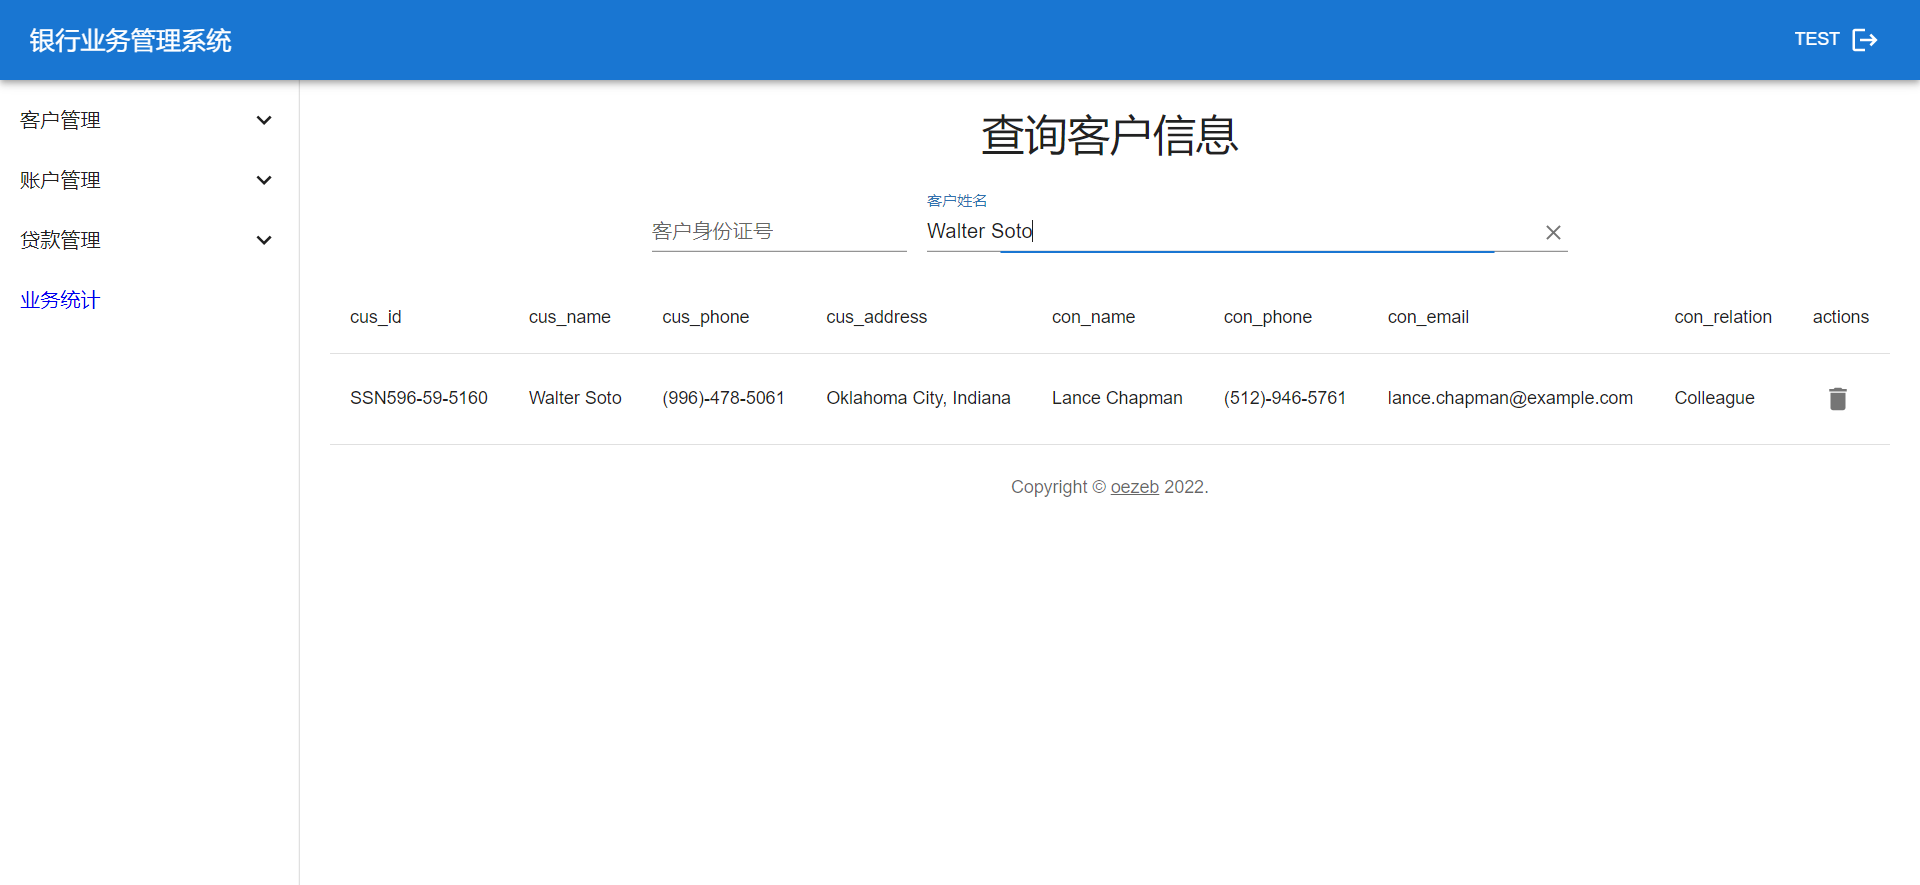
\includegraphics[width=\textwidth]{assets/images/customer-info.png}
        \end{figure}
    \end{enumerate}

    \item 账户管理模块
    
    \begin{enumerate}
        \item 开设账户模块 ("/open-account")
        
        给一定的客户开设一个支票或储蓄账户。
        
        \begin{figure}[H]
            \centering
            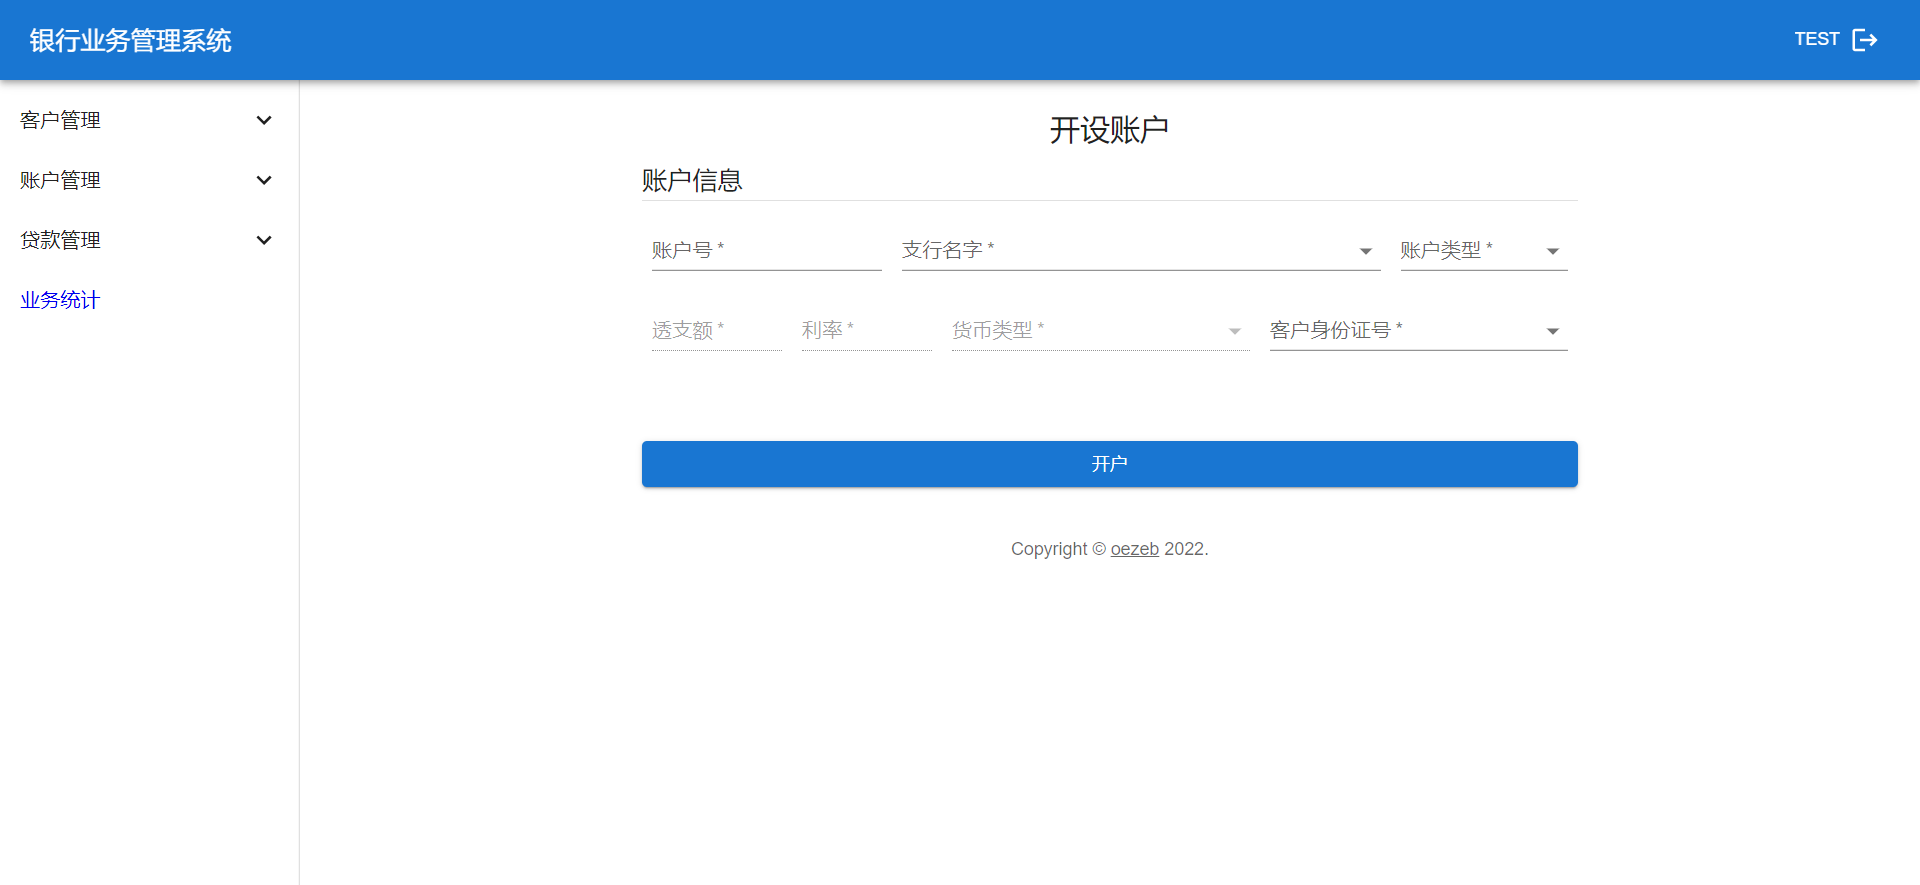
\includegraphics[width=\textwidth]{assets/images/open-account.png}
        \end{figure}

        \item 修改账户信息模块 ("/edit-account")
        
        选择账户后,其信息自动填充到表单中。修改账户信息,并提交。
        
        \begin{figure}[H]
            \centering
            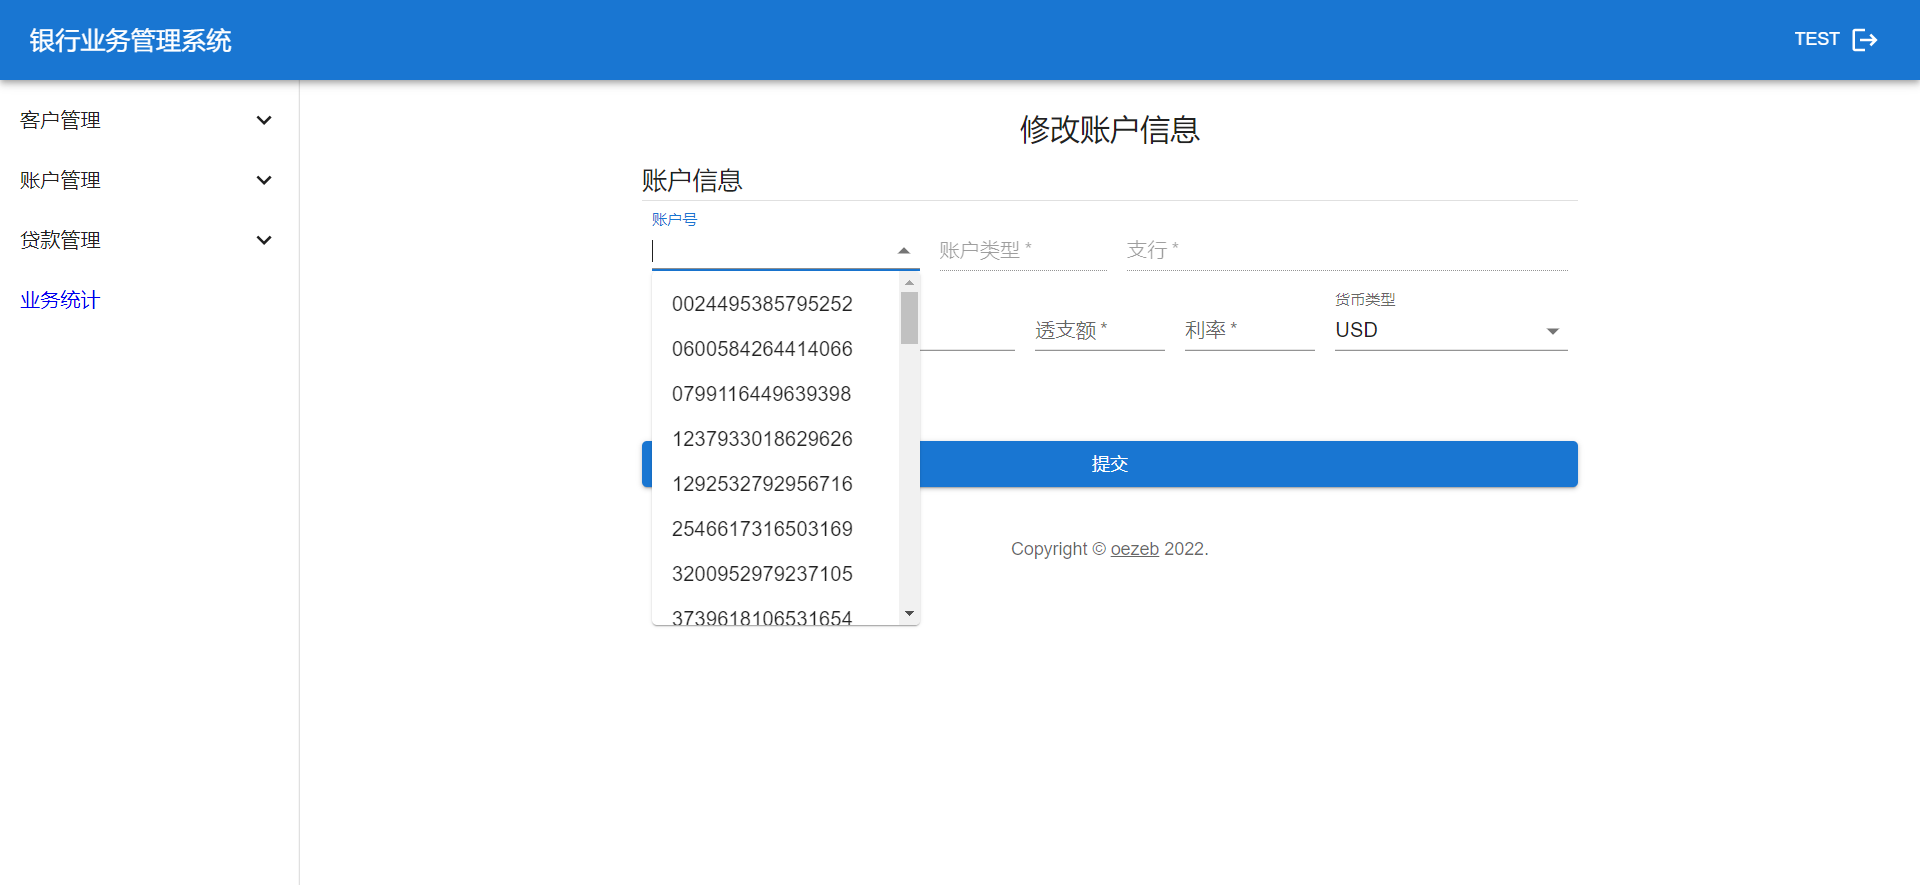
\includegraphics[width=\textwidth]{assets/images/edit-account.png}
        \end{figure}

        \item 查询账户信息模块 ("/account-info")
        
        根据账户号或客户身份证号或支行名称查询账户信息。结果列表中可以通过“actions”列的按钮删除账户。
        
        \begin{figure}[H]
            \centering
            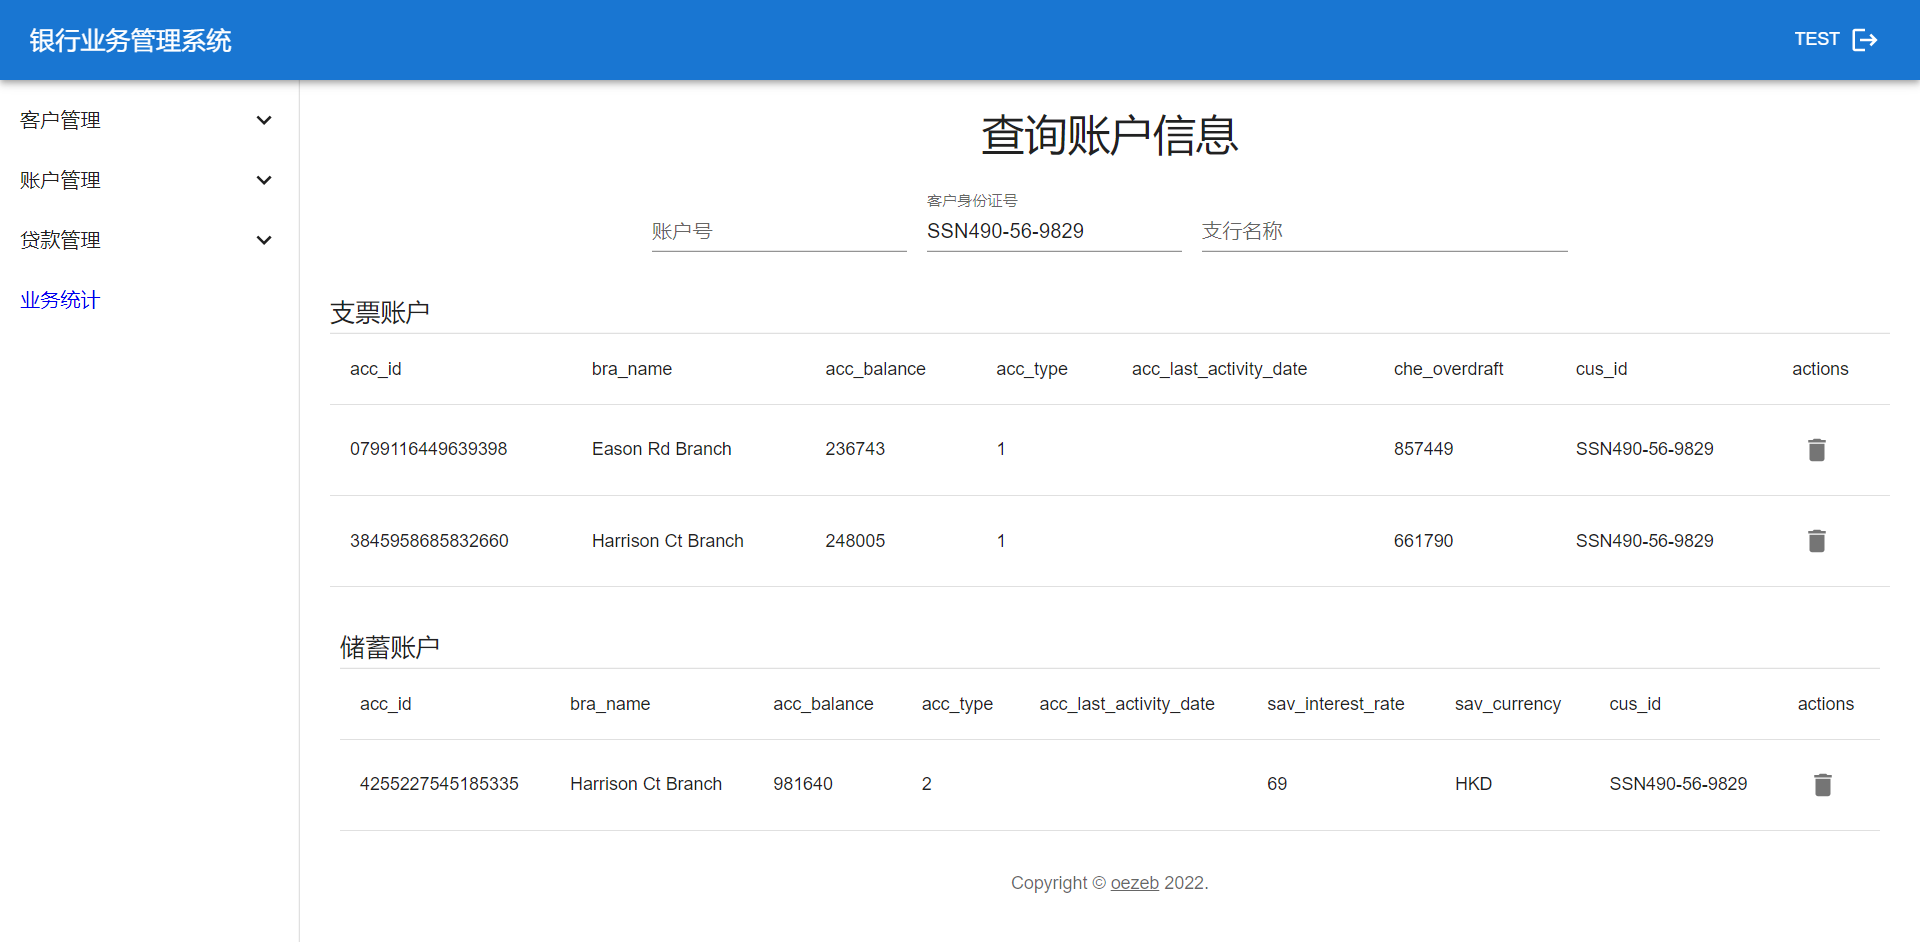
\includegraphics[width=\textwidth]{assets/images/account-info.png}
        \end{figure}
    \end{enumerate}


    \item 贷款管理模块
    
    \begin{enumerate}
        \item 增加贷款模块 ("/add-loan")
        
        填贷款信息,并提交。

        \begin{figure}[H]
            \centering
            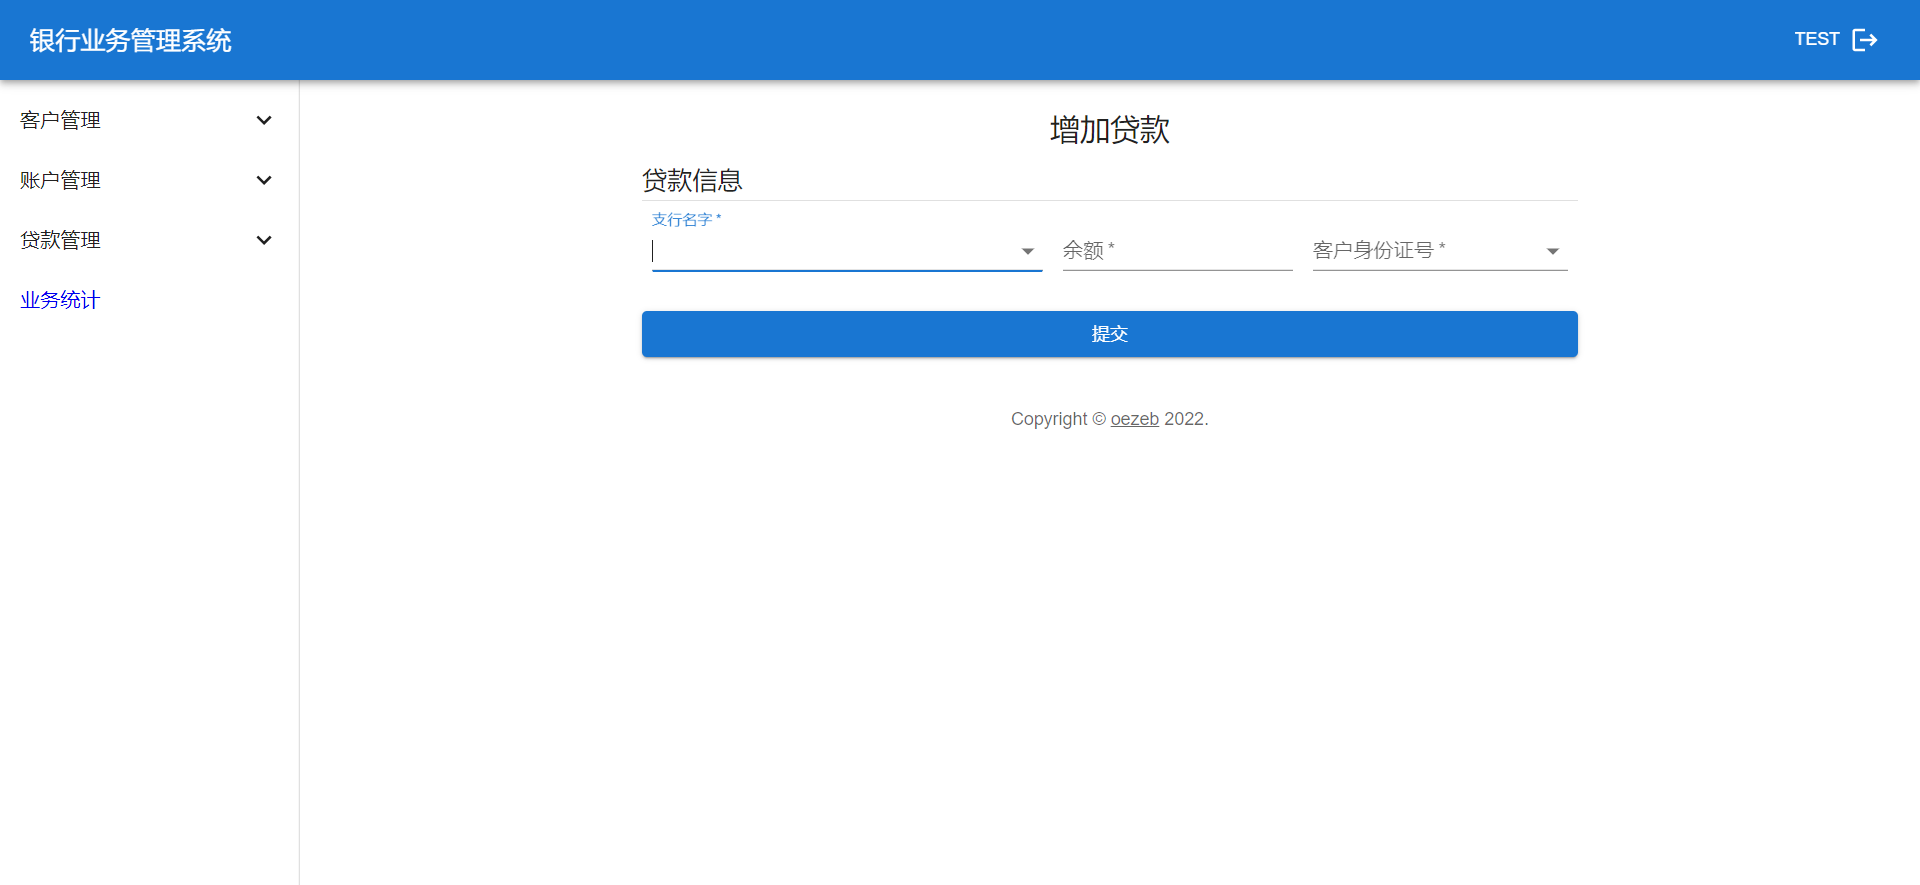
\includegraphics[width=\textwidth]{assets/images/add-loan.png}
        \end{figure}

        \item 发放贷款模块 ("/pay-loan")
        
        选择贷款后,其信息自动填充到表单中而且支付贷款的记录自动列出。 填写支付贷款的信息,并提交。
        
        \begin{figure}[H]
            \centering
            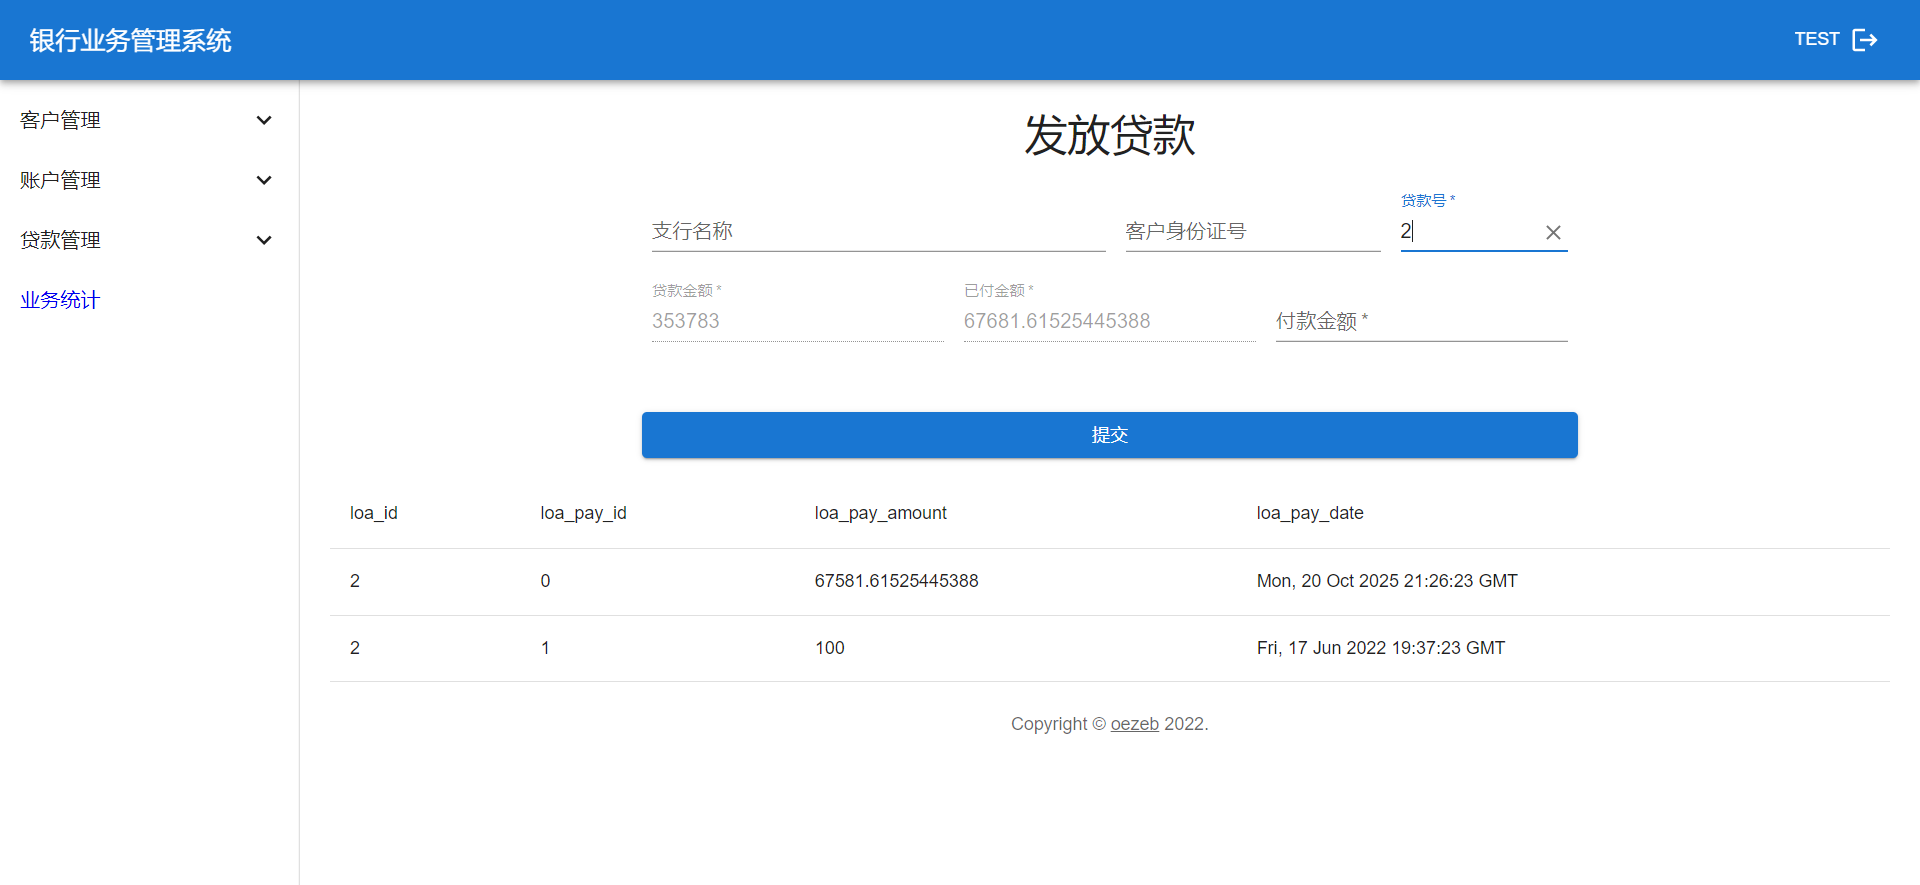
\includegraphics[width=\textwidth]{assets/images/pay-loan.png}
        \end{figure}

        \item 查询贷款信息模块 ("/loan-info")

        根据贷款号或客户身份证号或支行名称查询贷款信息。结果列表中可以通过“actions”列的按钮删除贷款。

        \begin{figure}[H]
            \centering
            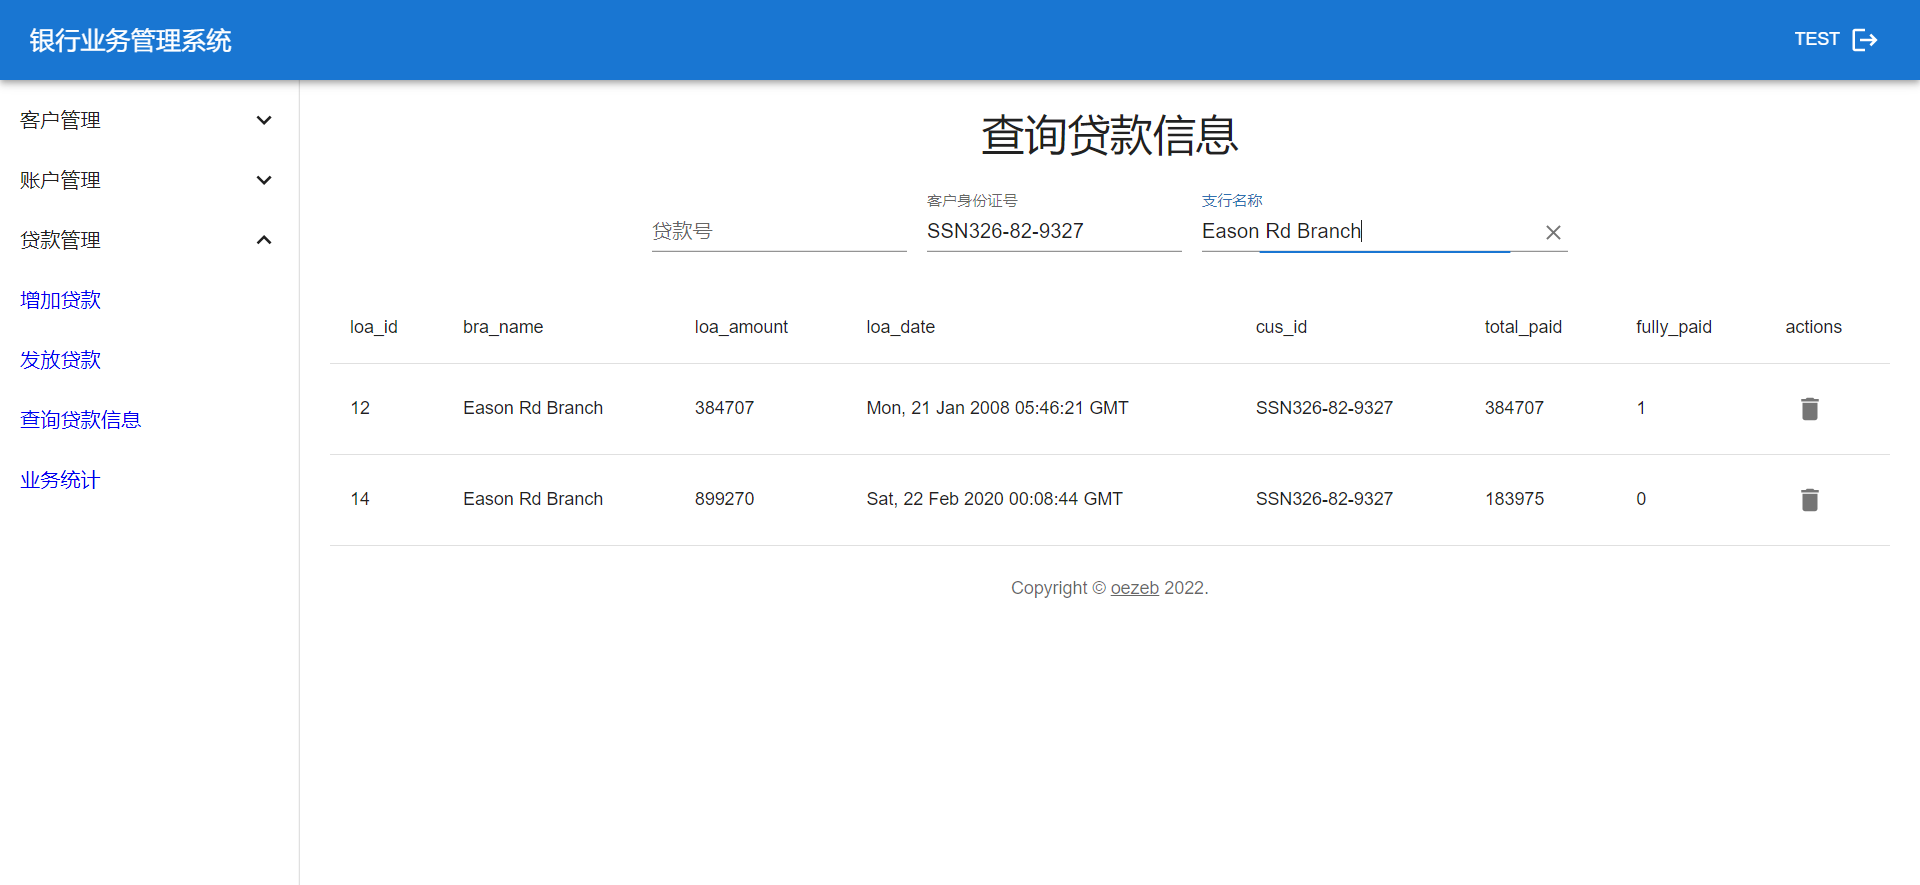
\includegraphics[width=\textwidth]{assets/images/loan-info.png}
        \end{figure}
    \end{enumerate}
\end{enumerate}


\section{总结与讨论}

本系统开发过程中, 从前端到后端学习了不少框架, 模块和语言, 例如 HTML, JavaScript, React, Flask, pymysql, MySQL DBMS 等. 这是大学期间少有的全栈开发工程经历, 非常有意义. 它不仅锻炼了系统设计能力, 也考验了我的工程实现能力, 更磨砺了我的耐心. 不得不说, 收获很大.

\end{document}
